
\section{Preliminary  Comparisons}
\label{Sec:Comparison}
\subsection{Performance profiles}
\frame{
  \frametitle{Performance profiles~\cite{Dolan.More2002}}

  \begin{itemize}
  \item Given a set of problems $\mathcal P$
  \item Given a set of solvers $\mathcal S$  
  \item A performance measure for each problem  with a solver $t_{p,s}$ (cpu time, flops, ...)
  \item Compute the performance ratio
    \begin{equation}
      \label{eq:perf-ratio}
      \tau_{p,s} =    \Frac{t_{p,s}}{\min_{s\in\mathcal S} t_{p,s}} \geq 1
    \end{equation}
  \item Compute the performance profile $\rho_s(\tau) : [1,+\infty]\rightarrow [0,1]$ for each solver $s\in \mathcal S$
    
    \begin{equation}
      \rho_s(\tau) = \Frac{1}{|\mathcal P|}\big|\{p\in \mathcal P\mid \tau_{p,s} \leq \tau    \}\big|\label{eq:perf}
  \end{equation}
  The value of $\rho_s(1)$ is the probability that the solver $s$ will win over the rest of the solvers.
  \end{itemize}
  
  
}
\def\ssep{1.5mm}

\subsection{Chain}
\frame{
  \frametitle{First comparisons. Chain}
  \begin{block}
    {Hanging chain with initial velocity at the tip}
    code: Siconos
    $$ $$
    \begin{minipage}{0.39\linewidth}
      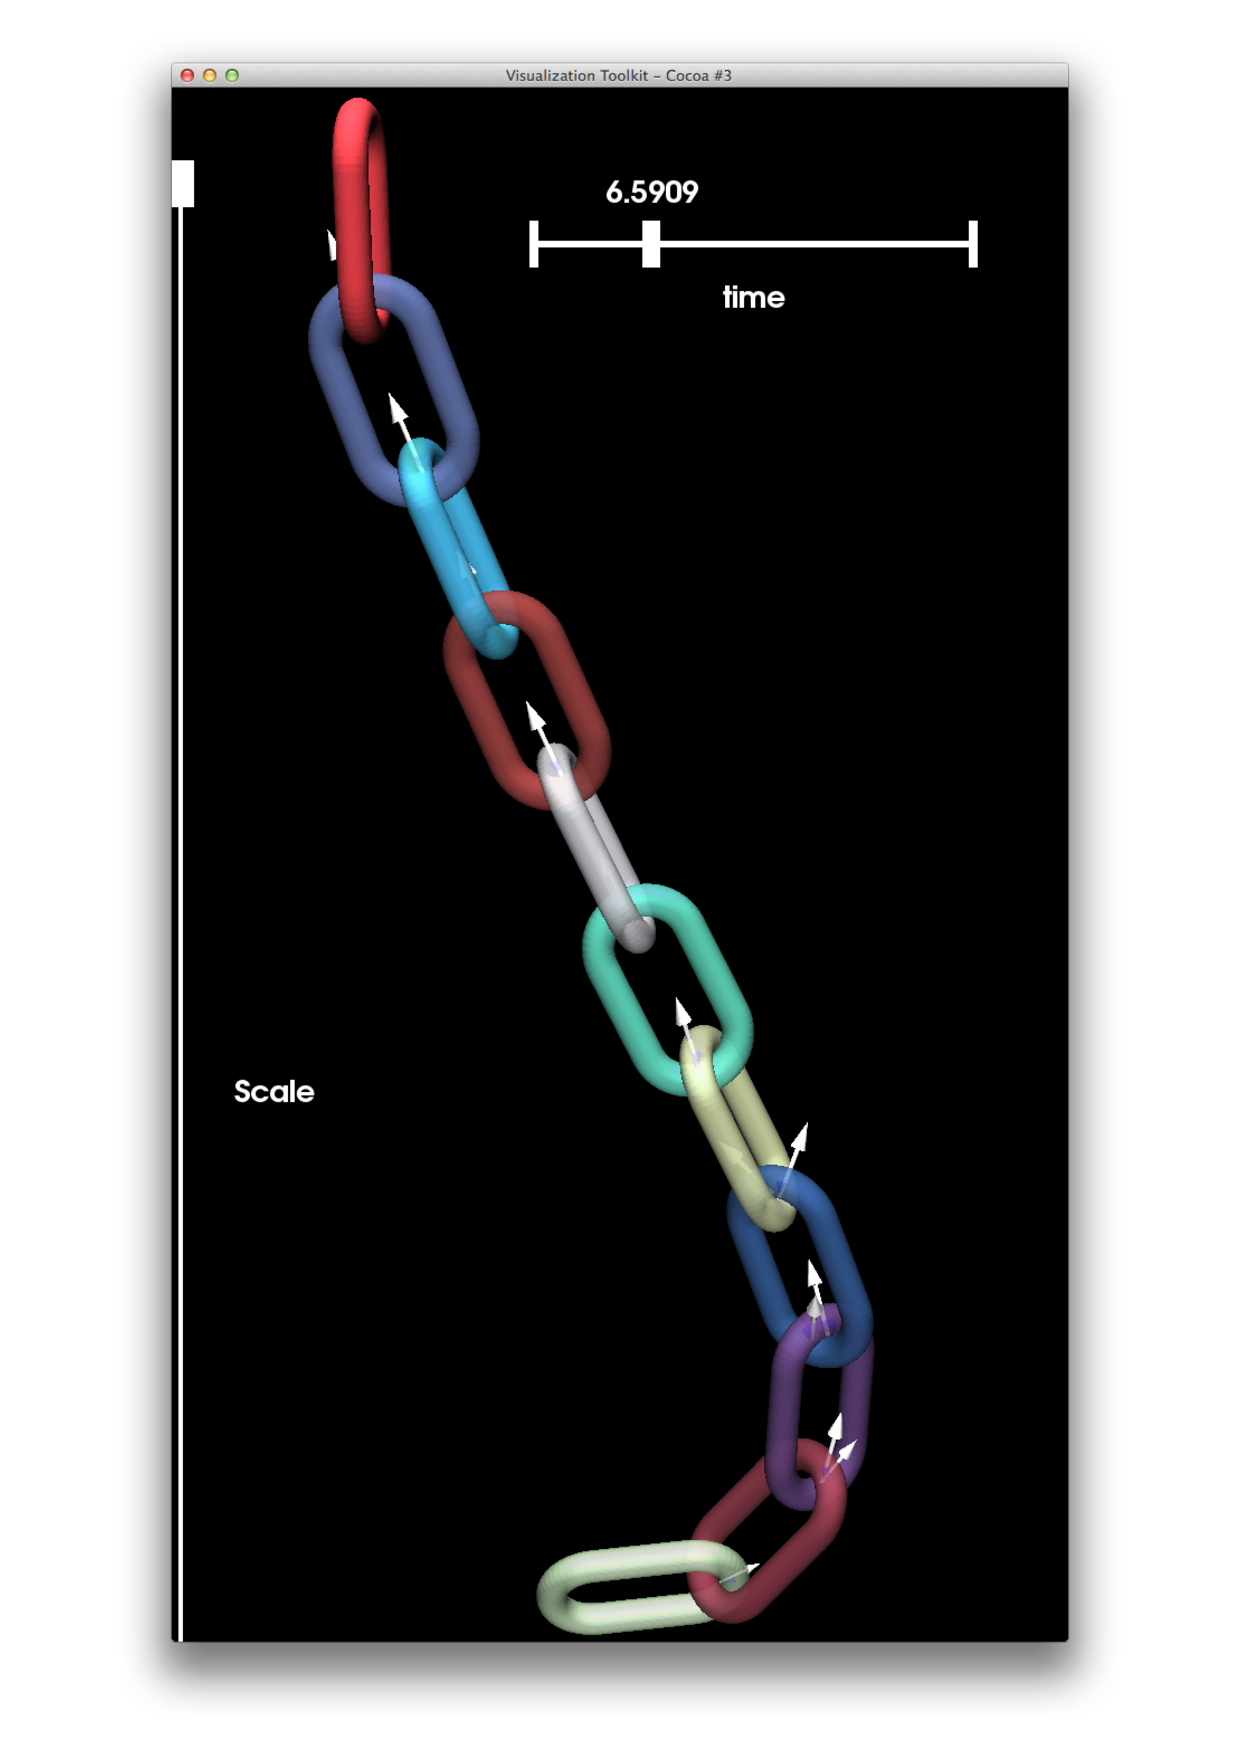
\includegraphics[width=1.0\textwidth]{Chains}
    \end{minipage}
    \begin{minipage}{0.49\linewidth}
      \begin{tabular}{|p{0.7\textwidth}|c|}
        coefficient of friction & $0.3$ \\[\ssep]
        number of problems & 1514 \\[\ssep]
        number of degrees of freedom & [48 : 60] \\[\ssep]
        number of contacts & [8 :28] \\[\ssep]
        required accuracy   & $10^{-8}$    
      \end{tabular}
    \end{minipage}
  \end{block}

}
\frame{
  \frametitle{First comparisons. Chain}
  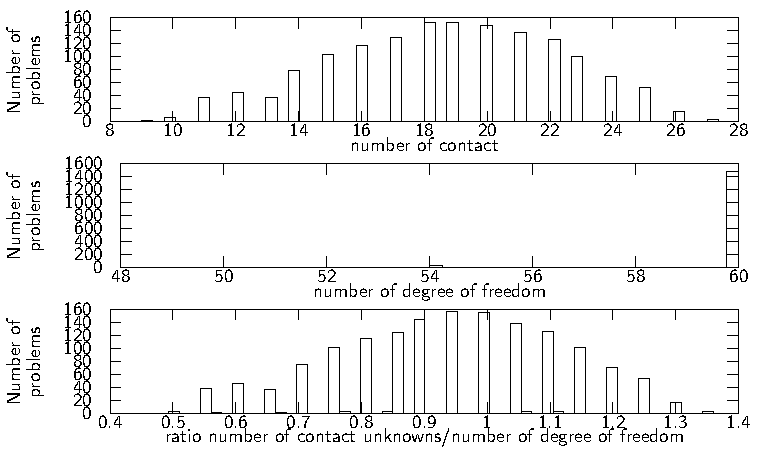
\includegraphics[width=1.10\textwidth]{distrib-Chain.pdf}
}
\frame{
  \frametitle{First comparisons. Chain}
    \centerline{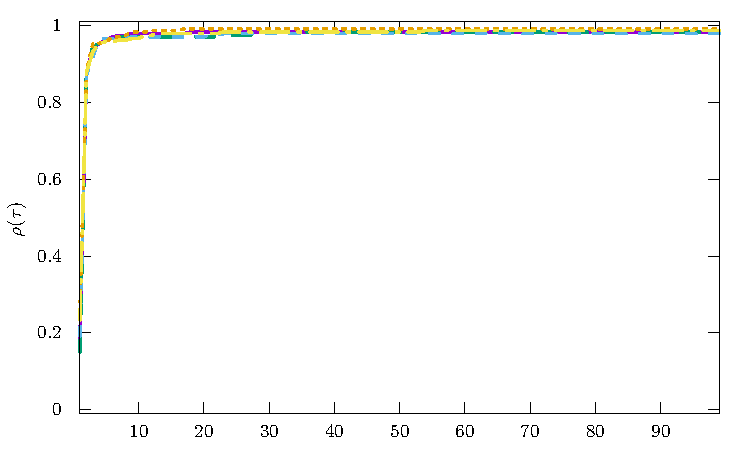
\includegraphics[width=0.7\textwidth]{COMP/large/flpops/profile-Chain.pdf}}
    \centerline{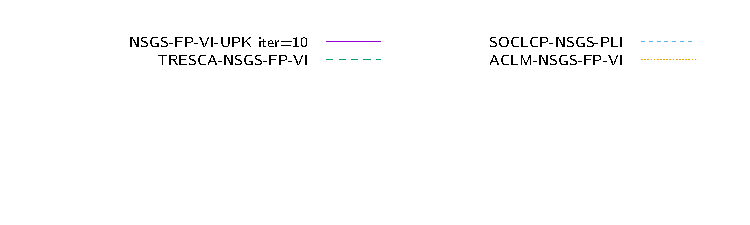
\includegraphics[width=0.7\textwidth]{COMP/large/flpops/profile-Chain_legend.pdf}}
}

\subsection{Capsules}

\frame{
  \frametitle{First comparisons. Capsules}
 \begin{block}
    {100 capsules dropped into a box.}
    code: Siconos
    $$ $$
  \begin{minipage}{0.49\linewidth}
    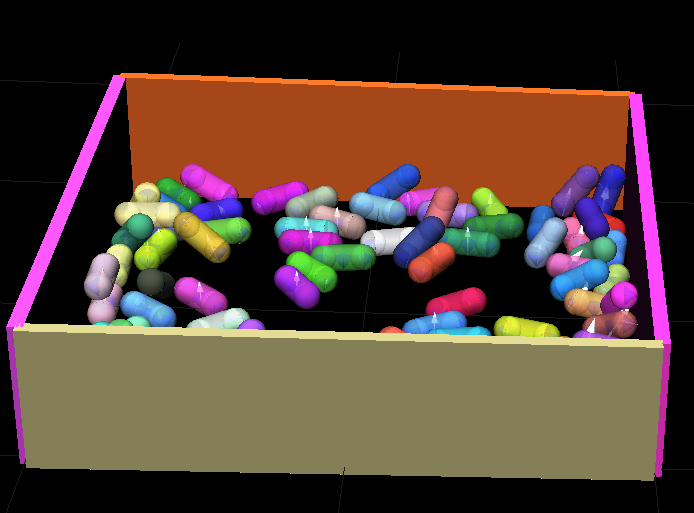
\includegraphics[width=1.0\textwidth]{Capsules}
  \end{minipage}  
  \begin{minipage}{0.49\linewidth}
    \begin{tabular}{|p{0.7\textwidth}|c|}
      coefficient of friction & $0.7$ \\[\ssep]
      number of problems & 1705 \\[\ssep]
      number of degrees of freedom & [6 : 600] \\[\ssep]
      number of contacts &  [0:300]\\[\ssep]
      required accuracy   & $10^{-8}$    
    \end{tabular}
  \end{minipage}
\end{block}
}
\frame{
  \frametitle{First comparisons. Capsules}
  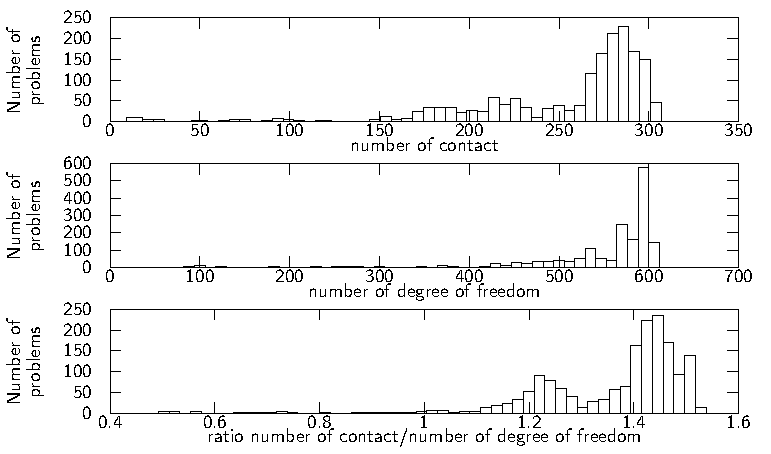
\includegraphics[width=1.10\textwidth]{distrib-Capsules.pdf}
}
% \frame{
%   \frametitle{First comparisons. Capsules}
%   \centerline{\includegraphics[width=1.10\textwidth]{profile-Capsules.pdf}}
% }
\frame{
  \frametitle{First comparisons. Capsules}
    \centerline{\includegraphics[width=0.7\textwidth]{COMP/large/flpops/profile-Capsules.pdf}}
    \centerline{
\includegraphics[width=0.7\textwidth]{COMP/large/flpops/profile-Capsules_legend.pdf}}
}




\subsection{Performance profiles. BoxesStack}

\frame{
  \frametitle{First comparisons. BoxesStack}
  \begin{block}
    {50 boxes stacked under gravity.}
    code: Siconos
    $$ $$
  \begin{minipage}{0.14\linewidth}
    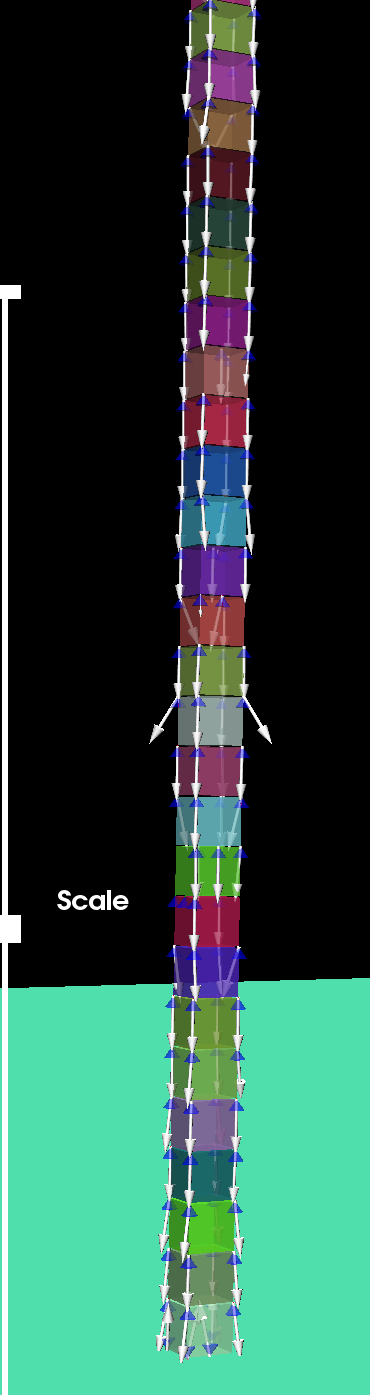
\includegraphics[width=1.0\textwidth]{BoxesStack}
  \end{minipage}
  \begin{minipage}{0.25\linewidth}
    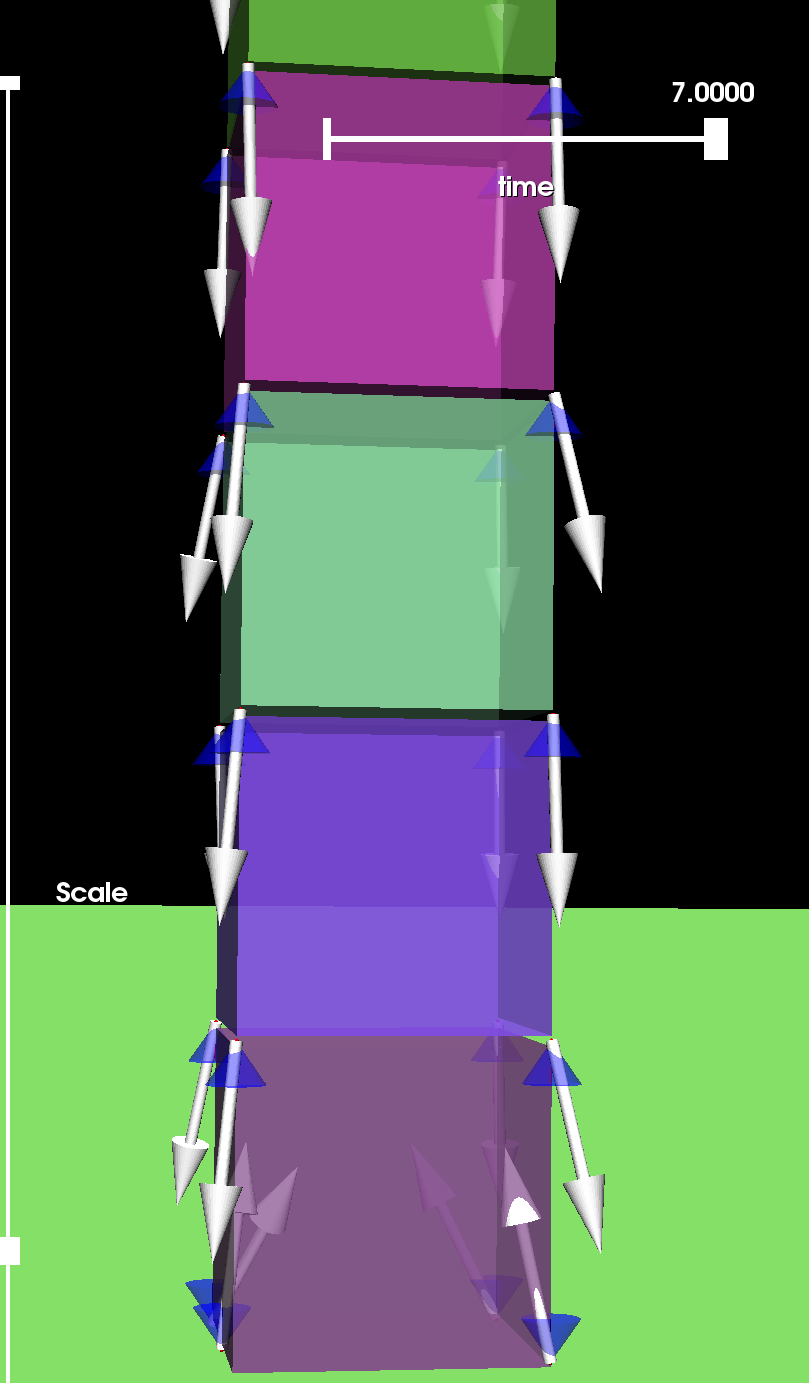
\includegraphics[width=1.0\textwidth]{BoxesStack2}
  \end{minipage}
  \begin{minipage}{0.49\linewidth}
    \begin{tabular}{|p{0.7\textwidth}|c|}
      coefficient of friction &  0.7\\[\ssep]
      number of problems &  1159 \\[\ssep]
      number of degrees of freedom & [6 : 300] \\[\ssep]
      number of contacts &  [ 0: 200]\\[\ssep]
      required accuracy   & $10^{-8}$
    \end{tabular}
  \end{minipage}
\end{block}
}
\frame{
  \frametitle{First comparisons. BoxesStack}
  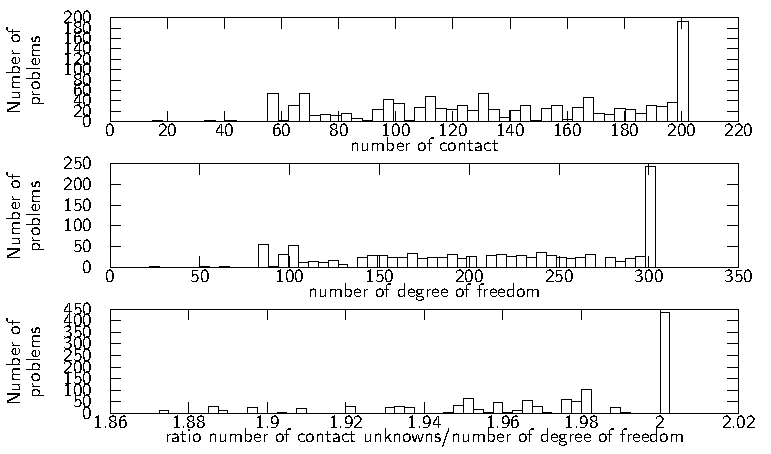
\includegraphics[width=1.10\textwidth]{distrib-BoxesStack1.pdf}
}
% \frame{
%   \frametitle{First comparisons. BoxesStack}
%   \centerline{\includegraphics[width=1.1\textwidth]{profile-BoxesStack1.pdf}}
% }
\frame{
  \frametitle{First comparisons. BoxesStack1}
    \centerline{\includegraphics[width=0.7\textwidth]{COMP/large/flpops/profile-BoxesStack1.pdf}}
    \centerline{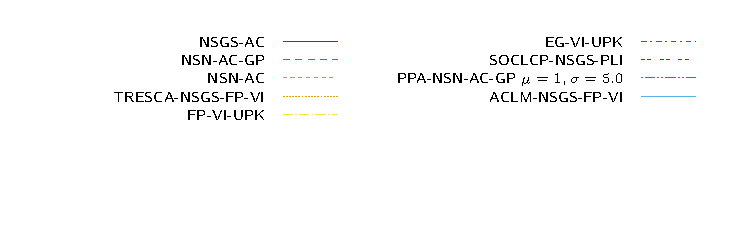
\includegraphics[width=0.7\textwidth]{COMP/large/flpops/profile-BoxesStack1_legend.pdf}}
}


\subsection{Performance profiles. Kaplas}

\frame{
  \frametitle{A tower of Kaplas}
  \begin{block}
    {A Tower of Kaplas}
    code: Siconos
    $$ $$
  \begin{minipage}{0.50\linewidth}
    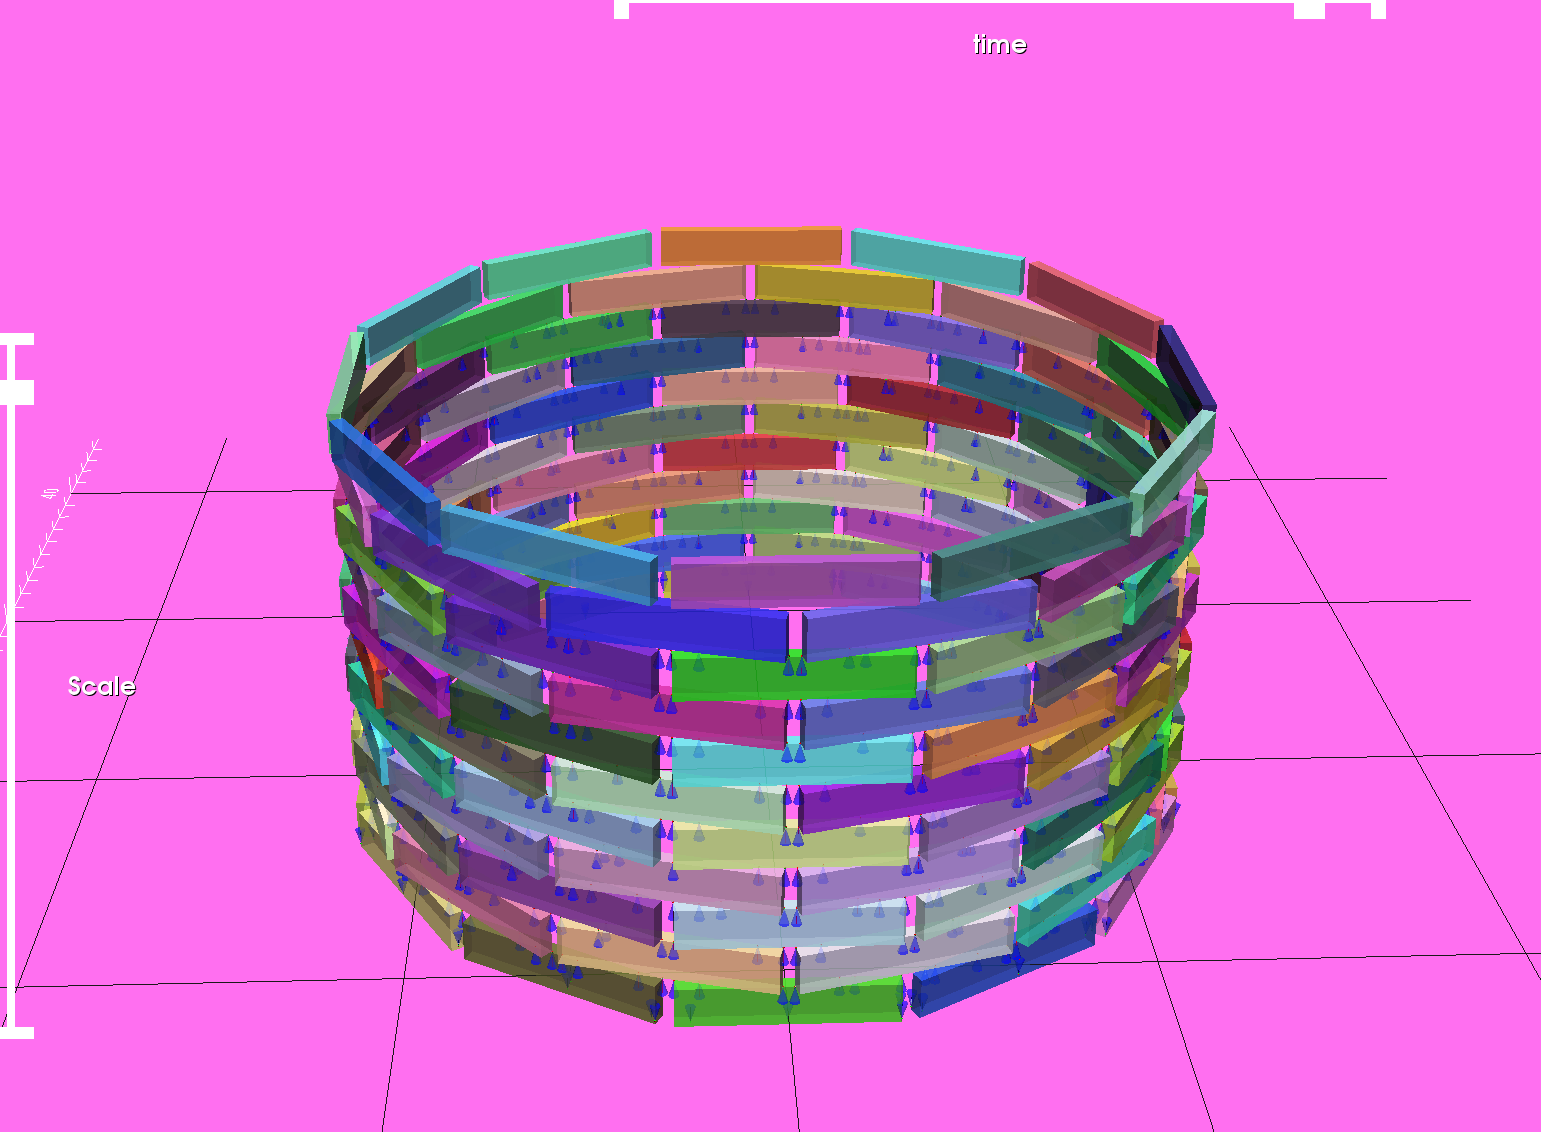
\includegraphics[width=1.0\textwidth]{KaplasTower}
  \end{minipage}
  \begin{minipage}{0.49\linewidth}
    \begin{tabular}{|p{0.7\textwidth}|c|}
      coefficient of friction &  0.3\\[\ssep]
      number of problems &  201 \\[\ssep]
      number of degrees of freedom & [72 : 864] \\[\ssep]
      number of contacts &  [ 0: 950]\\[\ssep]
      required accuracy   & $10^{-8}$
    \end{tabular}
  \end{minipage}
\end{block}
}
\frame{
  \frametitle{A tower of Kaplas}
  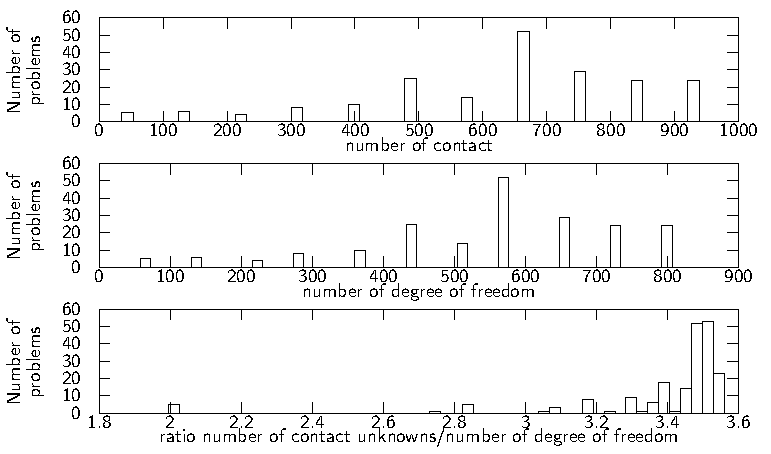
\includegraphics[width=1.10\textwidth]{distrib-KaplasTower.pdf}
}
% \frame{
%   \frametitle{A tower of  Kaplas}
%   \centerline{\includegraphics[width=1.1\textwidth]{profile-KaplasTower.pdf}}
% }
\frame{
  \frametitle{First comparisons. Kaplas Tower}
    \centerline{\includegraphics[width=0.7\textwidth]{COMP/large/flpops/profile-KaplasTower.pdf}}
    \centerline{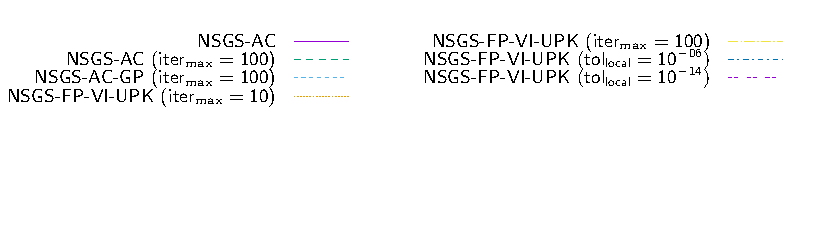
\includegraphics[width=0.7\textwidth]{COMP/large/flpops/profile-KaplasTower_legend.pdf}}
}
% \subsection{Performance profiles. AqueducPR}

% % \frame{An aqueduct}
% %   \begin{block}
% %     {An aqueduct}
% %     code: LMGC
% %     $$ $$
% %   \begin{minipage}{0.50\linewidth}
% %    % 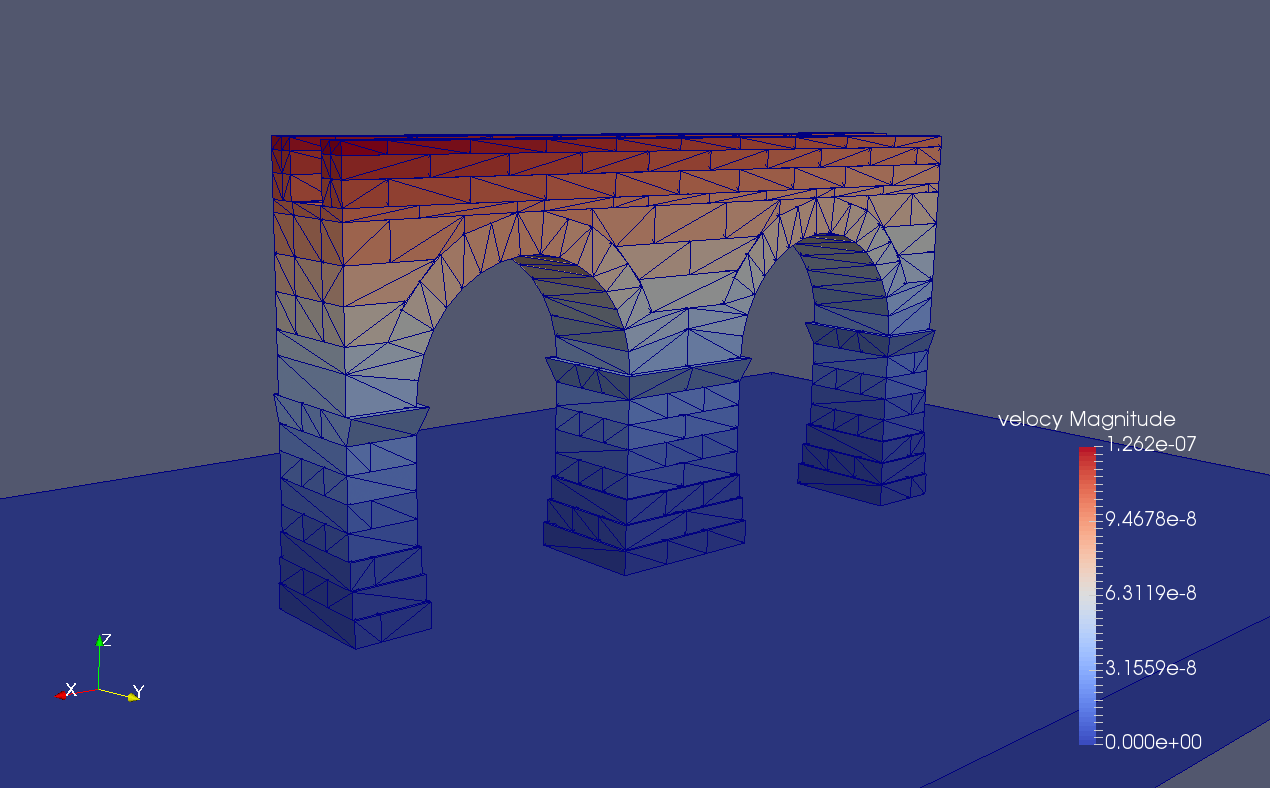
\includegraphics[width=1.0\textwidth]{Aqueduc_PR.png}
% %   \end{minipage}
% %   \begin{minipage}{0.49\linewidth}
% %     \begin{tabular}{|p{0.7\textwidth}|c|}
% %       coefficient of friction &  0.5\\[\ssep]
% %       number of problems &  10 \\[\ssep]
% %       number of degrees of freedom & 1932 \\[\ssep]
% %       number of contacts &  [ 4387: 4477]\\[\ssep]
% %       required accuracy   & $10^{-4}$
% %     \end{tabular}
% %   \end{minipage}
% % \end{block}
% % }
% % \frame{
% %   \frametitle{An aqueduct}
% %   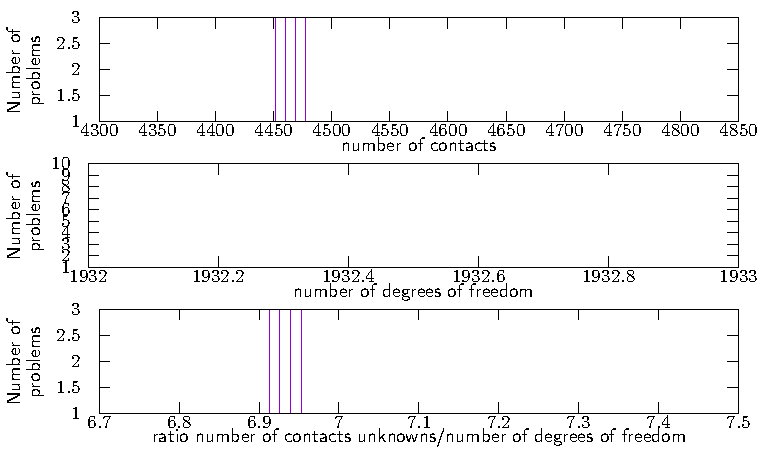
\includegraphics[width=1.10\textwidth]{distrib-LMGC_AqueducPR.pdf}
% % }
% % \frame{
% %   \frametitle{A tower of  Kaplas}
% %   \centerline{\includegraphics[width=1.1\textwidth]{profile-KaplasTower.pdf}}
% % }
% \frame{
%   \frametitle{First comparisons. An aqueduct}
%     \centerline{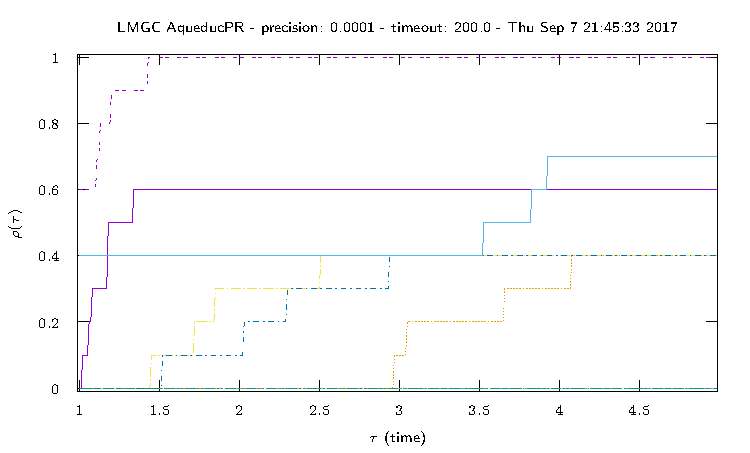
\includegraphics[width=0.7\textwidth]{COMP/large/flpops/profile-LMGC_AqueducPR.pdf}}
%     \centerline{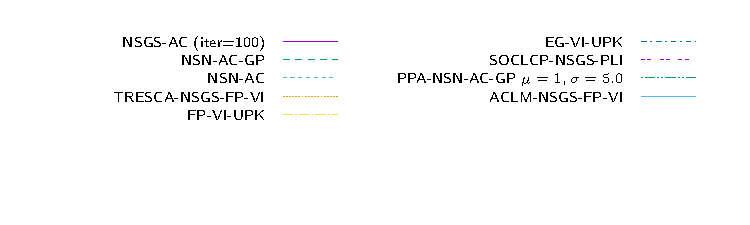
\includegraphics[width=0.7\textwidth]{COMP/large/flpops/profile-LMGC_AqueducPR_legend.pdf}}
% }





\subsection{Performance profiles.  FEM Cube H8}

\frame{
  \frametitle{Two elastic Cubes with FEM discretization H8}
  \begin{block}
    {Two elastic Cubes with FEM discretization H8}
    code : LMGC90
    $$ $$
   \begin{minipage}{0.40\linewidth}
     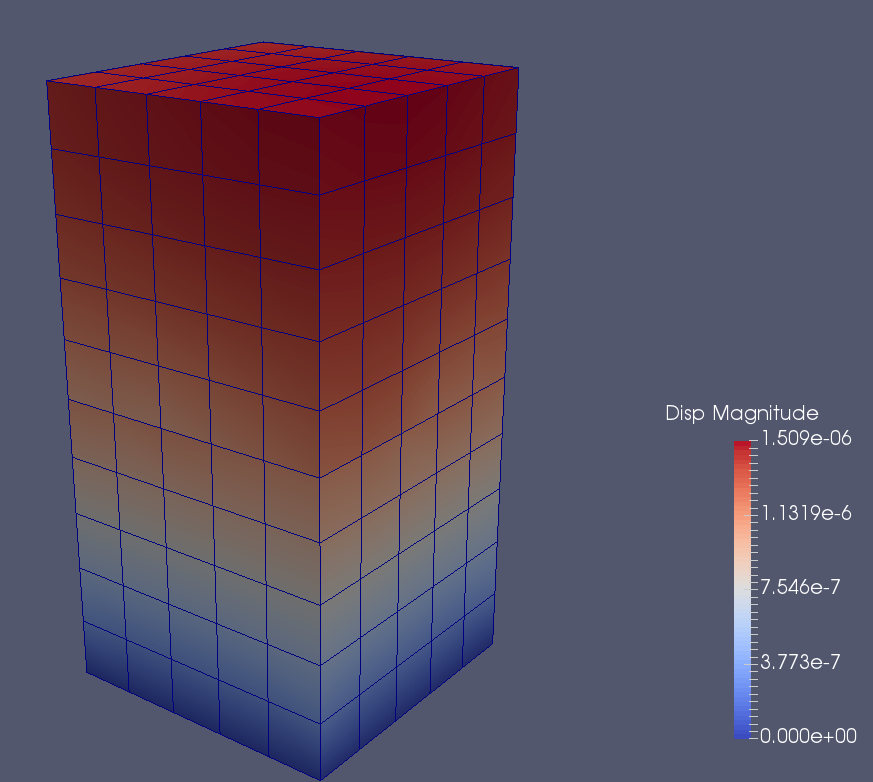
\includegraphics[width=1.0\textwidth]{Cubes_H8_5}
   \end{minipage}
   \begin{minipage}{0.49\linewidth}
     \begin{tabular}{|p{0.7\textwidth}|c|}
       coefficient of friction &  0.3\\[\ssep]
       number of problems &  58 \\[\ssep]
       number of degrees of freedom & \{162,1083,55566\} \\[\ssep]
       number of contacts &  [ 3:5] [30:36]  [360:368 ]\\[\ssep]
       required accuracy   & $10^{-5}$
     \end{tabular}
  \end{minipage}
\end{block}
}
\frame{
  \frametitle{Two elastic Cubes with FEM discretization H8}
  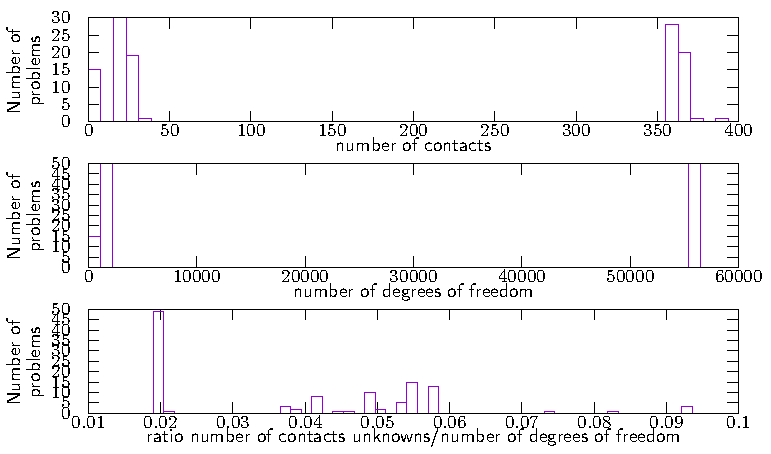
\includegraphics[width=1.10\textwidth]{distrib-LMGC_Cubes_H8_5.pdf}
 }
% \frame{
%   \frametitle{A tower of  Kaplas}
%   \centerline{\includegraphics[width=1.1\textwidth]{profile-KaplasTower.pdf}}
% }
\frame{
  \frametitle{First comparisons. Cubes H8}
    \centerline{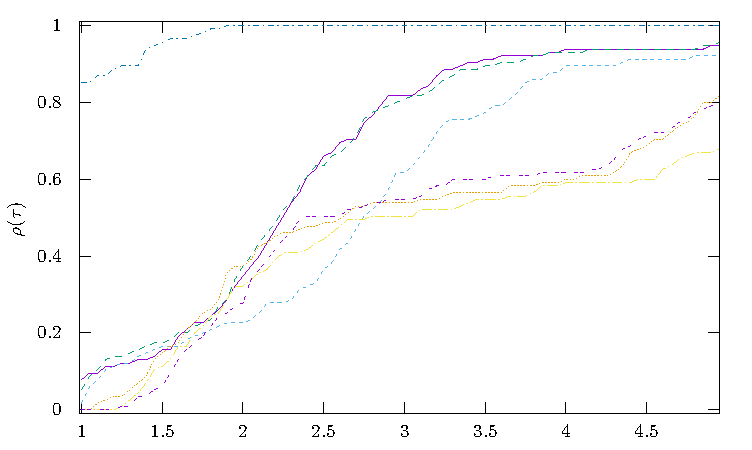
\includegraphics[width=0.7\textwidth]{COMP/large/flpops/profile-LMGC_Cubes_H8.pdf}}
    \centerline{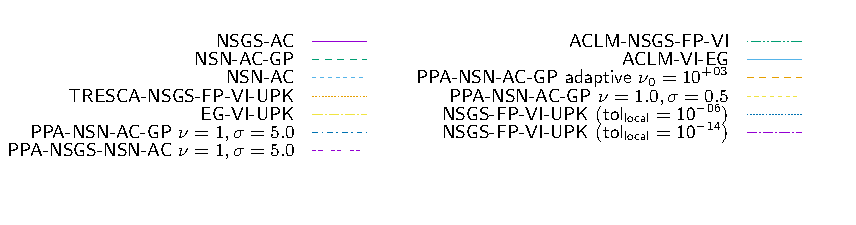
\includegraphics[width=0.7\textwidth]{COMP/large/flpops/profile-LMGC_Cubes_H8_legend.pdf}}
}



%%% Local Variables:
%%% mode: latex
%%% TeX-master: "s"
%%% End:

